\documentclass{article}
\usepackage {inputenc, fullpage, listings, amsmath, graphicx, amssymb, xcolor}

\parindent 0pt

\title{%
   ECE 260: Continuous-Time Signals and Systems\\
    Assignment 4\\
    }
\date{}

\begin{document}

\maketitle

\bigskip
{\bf 5.1 [find Fourier series]}\\
(a)
\begin{equation*}
\begin{split}
    x(t) &= 1 + cos(\pi t) + sin^2(\pi t)\\
    &= 1 + \frac{1}{2}(e^{j \pi t} + e^{-j \pi t}) + [\frac{1}{2j}(e^{j \pi t} - e^{-j \pi t})]^2\\
    &= 1 + \frac{1}{2}e^{j\pi t} + \frac{1}{2}e^{-j\pi t} - \frac{1}{4}((e^{j\pi t})^2 - 2(e^{j \pi t})(e^{-j\pi t}) + (e^{-j\pi t})^2)\\
    &= 1 + \frac{1}{2}e^{j \pi t} + \frac{1}{2}e^{-j \pi t} - \frac{1}{4}(e^{j 2 \pi t} - 2 + e^{-j 2 \pi t})\\
    &= -\frac{1}{4}e^{-j 2 \pi t} + \frac{1}{2}e^{-j \pi t} + \frac{3}{2} + \frac{1}{2}e^{j \pi t} - \frac{1}{4}e^{j 2 \pi t}
\end{split}
\end{equation*}

where $\omega_0 = \pi$
\begin{equation*}
\begin{split}
    c_k
    &= \begin{cases}
        \frac{3}{2} & k = 0\\
        \frac{1}{2} & k = \pm 1\\
        -\frac{1}{4} & k = \pm 2\\
        0 & otherwise
    \end{cases}\\
\end{split}
\end{equation*}

(c)\\
\begin{equation*}
\begin{split}
    T &= \frac{1}{2}\\
    \omega_0 &= \frac{2\pi}{1/2} = 4\pi
\end{split}
\end{equation*}

\begin{equation*}
\begin{split}
    c_k &= \frac{1}{T} \int_T x(t)e^{-jk\omega_0t}dt\\
    &= 2 \int_0^{1/2} |sin(2\pi t)|e^ {-jk4\pi t}dt\\
\end{split}
\end{equation*}
Since $\int e^{ax}sin(bx)dx = \frac{e^{ax}[asin(bx) - bcos(bx)]}{a^2 + b^2} + C$ where $a$ and $b$ are arbitrary complex and nonzero real constants, respectively.
\begin{equation*}
\begin{split}
    c_k &= 2[\frac{e^{-j4 \pi k t}[-j4 \pi ksin(2\pi t) - 2\pi cos(2 \pi t)]}{(-j4 \pi k)^2 + (2 \pi)^2}]\big|_0^{1/2}\\
    &= \frac{2(2 \pi)}{-16\pi^2 k^2 + 4\pi^2}[e^{-j4\pi kt} [-j2ksin(2 \pi) - cos(2\pi t)]]\big|_0^{1/2}\\
    &= \frac{1}{\pi(1-4k^2)}[e^{-j4\pi k/2} [-j2ksin(2 \pi / 2) - cos(2\pi t / 2)] + cos(0)]\\
    &= \frac{2}{\pi(1-4k^2)}
\end{split}
\end{equation*}


where $\omega_0 = 4\pi$
\begin{equation*}
\begin{split}
    c_k = \frac{2}{\pi(1 - 4k^2)}
\end{split}
\end{equation*}


\bigskip
{\bf 5.2 [find Fourier series]}\\
(a)\\
\begin{equation*}
\begin{split}
    T = 4 \text{ is the fundamental period, so } \omega_0 = \frac{2\pi}{T} = \frac{2\pi}{4} = \frac{\pi}{2}\\
\end{split}
\end{equation*}
\begin{equation*}
\begin{split}
    c_k &= \frac{1}{T} \int_T x(t)e^{-jk\omega_0t}dt\\
    &= \frac{1}{4} \int_{-2}^{2}[\delta(t - 1) - \frac{1}{2}\delta(t + 1)]e^{-j\pi kt/2}dt\\
    &= \frac{1}{4} \Big[\int_{-2}^{2}\delta(t - 1)e^{-j\pi kt/2}dt - \frac{1}{2}\int_{-2}^{2}\delta(t + 1)e^{-j\pi kt/2}dt\Big] \\
    &= \frac{1}{4}e^{-j \pi k/2} - \frac{1}{8}e^{j\pi k/2} \text{ sifting property}\\
    &= \frac{1}{4}(-j)^k - \frac{1}{8}j^k
\end{split}
\end{equation*}

\break
(c)\\
\begin{equation*}
\begin{split}
    T = 5 \text{ is the fundamental period, so } \omega_0 = \frac{2\pi}{T} = \frac{2\pi}{5}\\
\end{split}
\end{equation*}
\begin{equation*}
\begin{split}
    c_k &= \frac{1}{T} \int_T x(t)e^{-jk\omega_0t}dt\\  
    &= \frac{1}{5} \int_{-5/2}^{5/2} x(t) e^{-j 2 \pi kt/5}dt\\
    &= \frac{1}{5} \Big[\int_{-2}^{-1} e^{-j 2 \pi kt/5}dt + \int_{-1}^{1} 2e^{-j 2 \pi kt/5}dt + \int_{1}^{2} e^{-j 2 \pi kt/5}dt \Big]\\
    &= \frac{1}{5} \Big[\frac{1}{-j2\pi k/5}e^{-jk 2\pi t /5}\Big|_{-2}^{2} + \frac{2}{-j2\pi k/5}e^{-jk 2\pi t /5}\Big|_{-1}^{1} + \frac{1}{-j2\pi k/5}e^{-jk 2\pi t /5}\Big|_{1}^{2}\Big]\\
    &= \frac{1}{-j2\pi k} \Big[e^{-jk 2\pi t /5}\Big|_{-2}^{2} + 2e^{-jk 2\pi t /5}\Big|_{-1}^{1} + e^{-jk 2\pi t /5}\Big|_{1}^{2}\Big]\\
    &= \frac{1}{-j2\pi k} [ e^{-jk 2\pi (-1) /5} - e^{-jk 2\pi (-2) /5} + 2e^{-jk 2\pi (1) /5} - 2e^{-jk 2\pi (-1) /5} + e^{-jk 2\pi (2) /5} - e^{-jk 2\pi (1) /5} ]\\
    &= \frac{1}{-j2\pi k} [ e^{jk 2\pi /5} - e^{2jk 2\pi /5} + 2e^{-jk 2\pi /5} - 2e^{jk 2\pi /5} + e^{-2jk 2\pi /5} - e^{-jk 2\pi /5} ]\\
    &= \frac{1}{-j2\pi k} [ e^{-j4\pi k/5} - e^{j4\pi k/5} + e^{-j2\pi k/5} - e^{j2\pi k/5}]\\
    &= \frac{1}{-j2\pi k} [-2jsin(4 \pi k/5) - 2jsin(2 \pi k/5)]\\
    &= \frac{1}{\pi k} [sin(4 \pi k/5) - sin(2 \pi k/5)]\\
    &= \frac{sin(4 \pi k/5)}{\pi k} + \frac{sin(2 \pi k/5)}{\pi k}\\
    &= \frac{4}{5} sinc(4 \pi k/5) + \frac{2}{5} sinc(2 \pi k/5) \text{ for $k = 0$}\\
\end{split}
\end{equation*}

\begin{equation*}
\begin{split}
    \text{For } k &= 0\\
    c_k &= \frac{1}{T} \int_T x(t)\\  
    &= \frac{1}{5} \int_{-5/2}^{5/2} x(t)\\
    &= \frac{1}{5} \Big[ \int_{-2}^{-1}dt + \int_{-1}^{1}2dt + \int_{1}^{2}dt \Big]\\
    &= \frac{1}{5} [-1-(-2) + 2(1 - (-1)) + 2 - 1]\\
    &= \frac{1}{5}(6)\\
    &= \frac{6}{5}
\end{split}
\end{equation*}

$\therefore$ we get:
\begin{equation*}
\begin{split}
    c_k
    &= \begin{cases}
        \frac{6}{5} & k = 0\\
        \frac{4}{5} sinc(4 \pi k/5) + \frac{2}{5} sinc(2 \pi k/5) & \text{otherwise}\\
    \end{cases}\\
\end{split}
\end{equation*}


\bigskip
{\bf 5.6 [odd harmonic proof]}\\
(b)
\begin{equation*}
\begin{split}
    x(t) &= \sum_{k = -\infty}^{\infty}c_ke^{jk\omega_0t}\\
    -x(t=\frac{T}{2}) &= -\sum_{k = -\infty}^{\infty}c_ke^{-jk\omega_0(t-T/2)}\\
    &= -\sum_{k = -\infty}^{\infty}c_ke^{jk\omega_0t} e^{-jk\omega_0T/2}\\
    &= -\sum_{k = -\infty}^{\infty}c_ke^{jk\omega_0t} e^{-j\pi k}\\
    &= -\sum_{k = -\infty}^{\infty}(-1)^{k}c_k e^{jk\omega_0t}\\
    &= \sum_{k = -\infty}^{\infty}(-1)^{k + 1}c_k e^{jk\omega_0t}\\
    c_k &= (-1)^{k + 1}\\
    c_k
    &= \begin{cases}
        -c_k & even\\
        c_k & odd\\
    \end{cases}\\
\end{split}
\end{equation*}
$\therefore \; x$ is odd harmonic iff $x(t) = -x(t - \frac{T}{2})$ for all $t$

\bigskip
{\bf 5.8 [find/plot frequency spectrum]}\\
\begin{equation*}
\begin{split}
    T = 2 \text{ is the fundamental period, so } \omega_0 = \frac{2\pi}{T} = \frac{2\pi}{2} = \pi\\
\end{split}
\end{equation*}

\begin{equation*}
\begin{split}
    c_k &= \frac{1}{T} \int_T x(t)e^{-jk\omega_0t}dt\\  
    &= \frac{1}{2} \int_0^2 x(t)e^{-j\pi kt}dt\\  
    &= \frac{1}{2} \int_0^1 e^{-j\pi kt}dt\\ 
    &= \frac{1}{2} \Big[\frac{1}{-j \pi k}e^{-j\pi k t}\Big]\Big|_{0}^{1}\\
    &= \frac{1}{2} \Big[\frac{1}{-j \pi k}e^{-j\pi k (1)} - \frac{1}{-j \pi k}e^{-j\pi k (0)}\Big]\\
    &= \frac{1}{j2\pi k}[1 - e^{-j\pi k}]\\
    &= \frac{1}{j2\pi k} [1-(-1)^k]\\
    c_k
    &= \begin{cases}
        -\frac{j}{\pi k} & k \text{ odd}\\
        0 & k \text{ even, } k \neq 0\\
    \end{cases}\\
\end{split}
\end{equation*}

\begin{equation*}
\begin{split}
    \text{if }k &= 0\\
    c_0 &= \frac{1}{T} \int_T x(t)dt \\ 
    &= \frac{1}{2} \int_{0}^{2} x(t)\\
    &= \frac{1}{2} \int_{0}^{1} dt\\
    &= \frac{1}{2}[t]\Big|_0^1\\
    &= \frac{1}{2}
\end{split}
\end{equation*}

\begin{equation*}
\begin{split}
     c_k
    &= \begin{cases}
        \frac{1}{2} & k = 0\\
        -\frac{j}{\pi k} & k \text{ odd}\\
        0 & k \text{ even, } k \neq 0\\
    \end{cases}\\
\end{split}
\end{equation*}

First Fourier series coefficients:
\begin{equation*}
\begin{split}
    k = 0, \; |c_k| &= \frac{1}{2}, \; arg(c_k) = 0\\
    k = 1, \; |c_k| &= \frac{1}{\pi}, \; arg(c_k) = -\frac{\pi}{2}\\
    k = 2, \; |c_k| &= 0, \; arg(c_k) = 0\\
    k = 3, \; |c_k| &= \frac{1}{3\pi}, \; arg(c_k) = -\frac{\pi}{2}\\
    k = 4, \; |c_k| &= 0, \; arg(c_k) = 0\\
    k = 5, \; |c_k| &= \frac{1}{5\pi}, \; arg(c_k) = -\frac{\pi}{2}\\
\end{split}
\end{equation*}

\begin{center}
    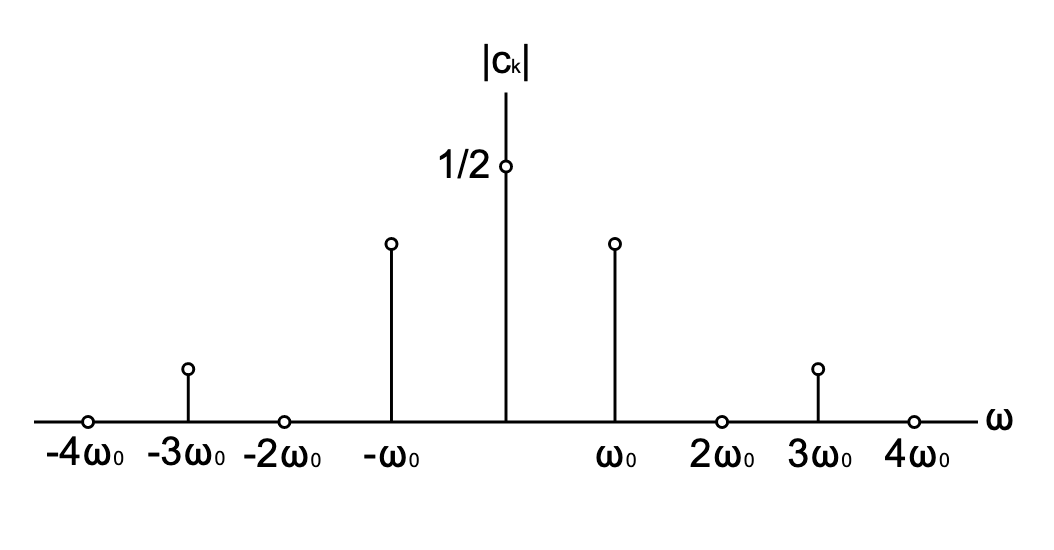
\includegraphics[width=0.5\textwidth]{581.png}
\end{center}

\begin{center}
    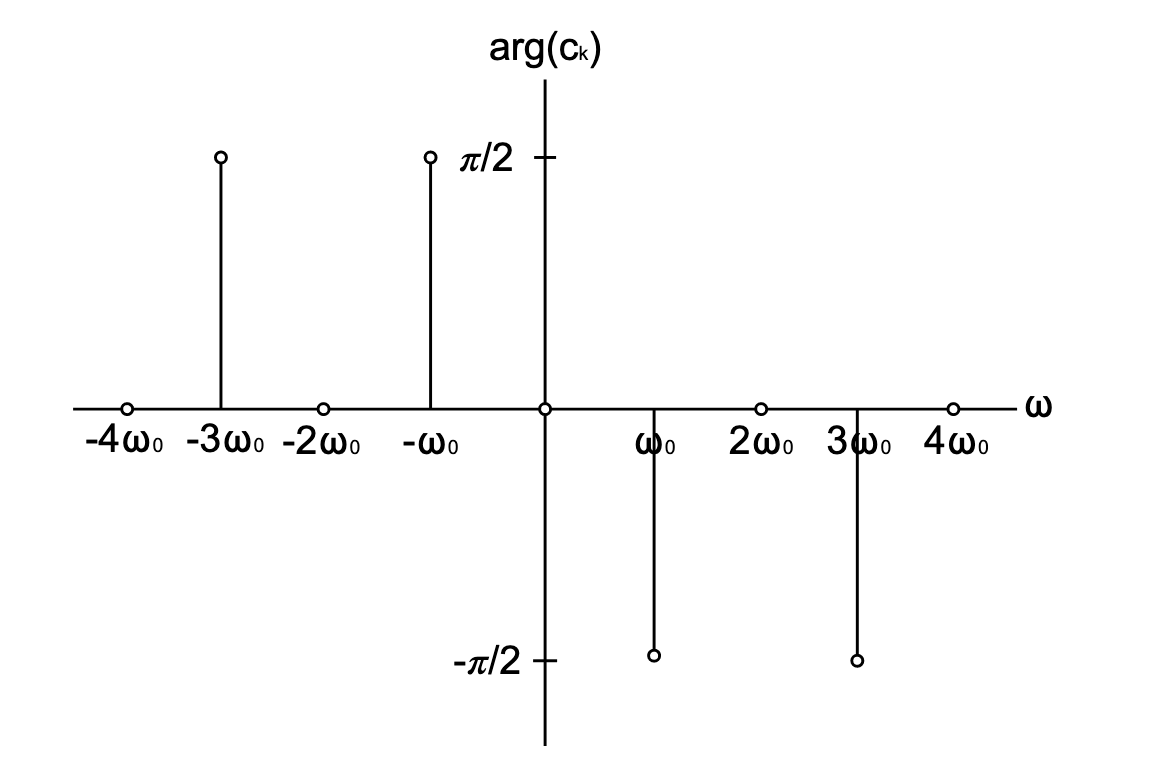
\includegraphics[width=0.5\textwidth]{582.png}
\end{center}

\bigskip
{\bf 5.9 [filtering]}\\
\begin{equation*}
\begin{split}
    x(t) &= 1 + 2cos(2t) + 2cos(4t) + \frac{1}{2}cos(6t)\\
    &= 1 + 2[\frac{1}{2}(e^{j2t} + e^{-j2t})] + 2[\frac{1}{2}(e^{j4t} + e^{-j4t})] + \frac{1}{2}[\frac{1}{2}(e^{j6t} + e^{-j6t})]\\
    &= 1 + e^{j2t} + e^{-j2t} + e^{j4t} + e^{-j4t} + e^{j6t} + e^{-j6t}\\
\end{split}
\end{equation*}

\begin{equation*}
\begin{split}
     c_k
    &= \begin{cases}
        1 & k = 0\\
        1 & k \pm 1\\
        1 & k \pm 2\\
        \frac{1}{4} & k \pm\\
        0 & otherwise\\
    \end{cases}\\
\end{split}
\end{equation*}

Since the system is LTI:
\begin{equation*}
\begin{split}
    y(t) = \sum_{k = -\infty}^{\infty} b_ke^{jk\omega_0 t}
\end{split}
\end{equation*}

\begin{equation*}
\begin{split}
    b_0 &= a_0H([0][2]]) = 0\\
    b_1 &= a_1H([1][2]]) = 0\\
    b_{-1} &= a_{-1}H([-1][2]]) = 0\\
    b_{2} &= a_{2}H([2][2]]) = 0\\
    b_{-2} &= a_{-2}H([-2][2]]) = 0\\
    b_{3} &= a_{3}H([3][2]]) = \frac{1}{4}\\
    b_{-3} &= a_{-3}H([-3][2]]) = \frac{1}{4}\\
\end{split}
\end{equation*}

\begin{equation*}
\begin{split}
     c_k
    &= \begin{cases}
        \frac{1}{4} & k = \pm 3\\
        0 & otherwise\\
    \end{cases}\\
\end{split}
\end{equation*}

$\therefore$ the output for $y$ is:
\begin{equation*}
\begin{split}
    y(t) &= \frac{1}{4}e^{-j6t} + \frac{1}{4}e^{j6t}\\
    &= \frac{1}{4}[e^{-j6t} + e^{j6t}]\\
    &= \frac{1}{4} [2cos(6t)]\\
    &= \frac{1}{2}cos(6t)\\
\end{split}
\end{equation*}


\bigskip
{\bf 5.101 [Fourier series convergence]}\\
(a)
\begin{lstlisting}
    syms t;
    delta = @(t) 1 - abs(-heaviside(-t) + heaviside(t));
    mysinc = @(t) (sin(t) + delta(t)) / (t + delta(t));
    A = 0.5;
    syms k;
    for nVal = [1 5 10 50 100]
        % op = -n
        f = symsum(0.5 * mysinc(pi / 2 * k) 
            * exp(j * k * (2 * pi) * t), k, -n, n);
        ezplot(f, [-1 1]); 
        title(sprintf('x_{%d}(t)', nVal));
        pause (2);
    end
\end{lstlisting}

\begin{center}
    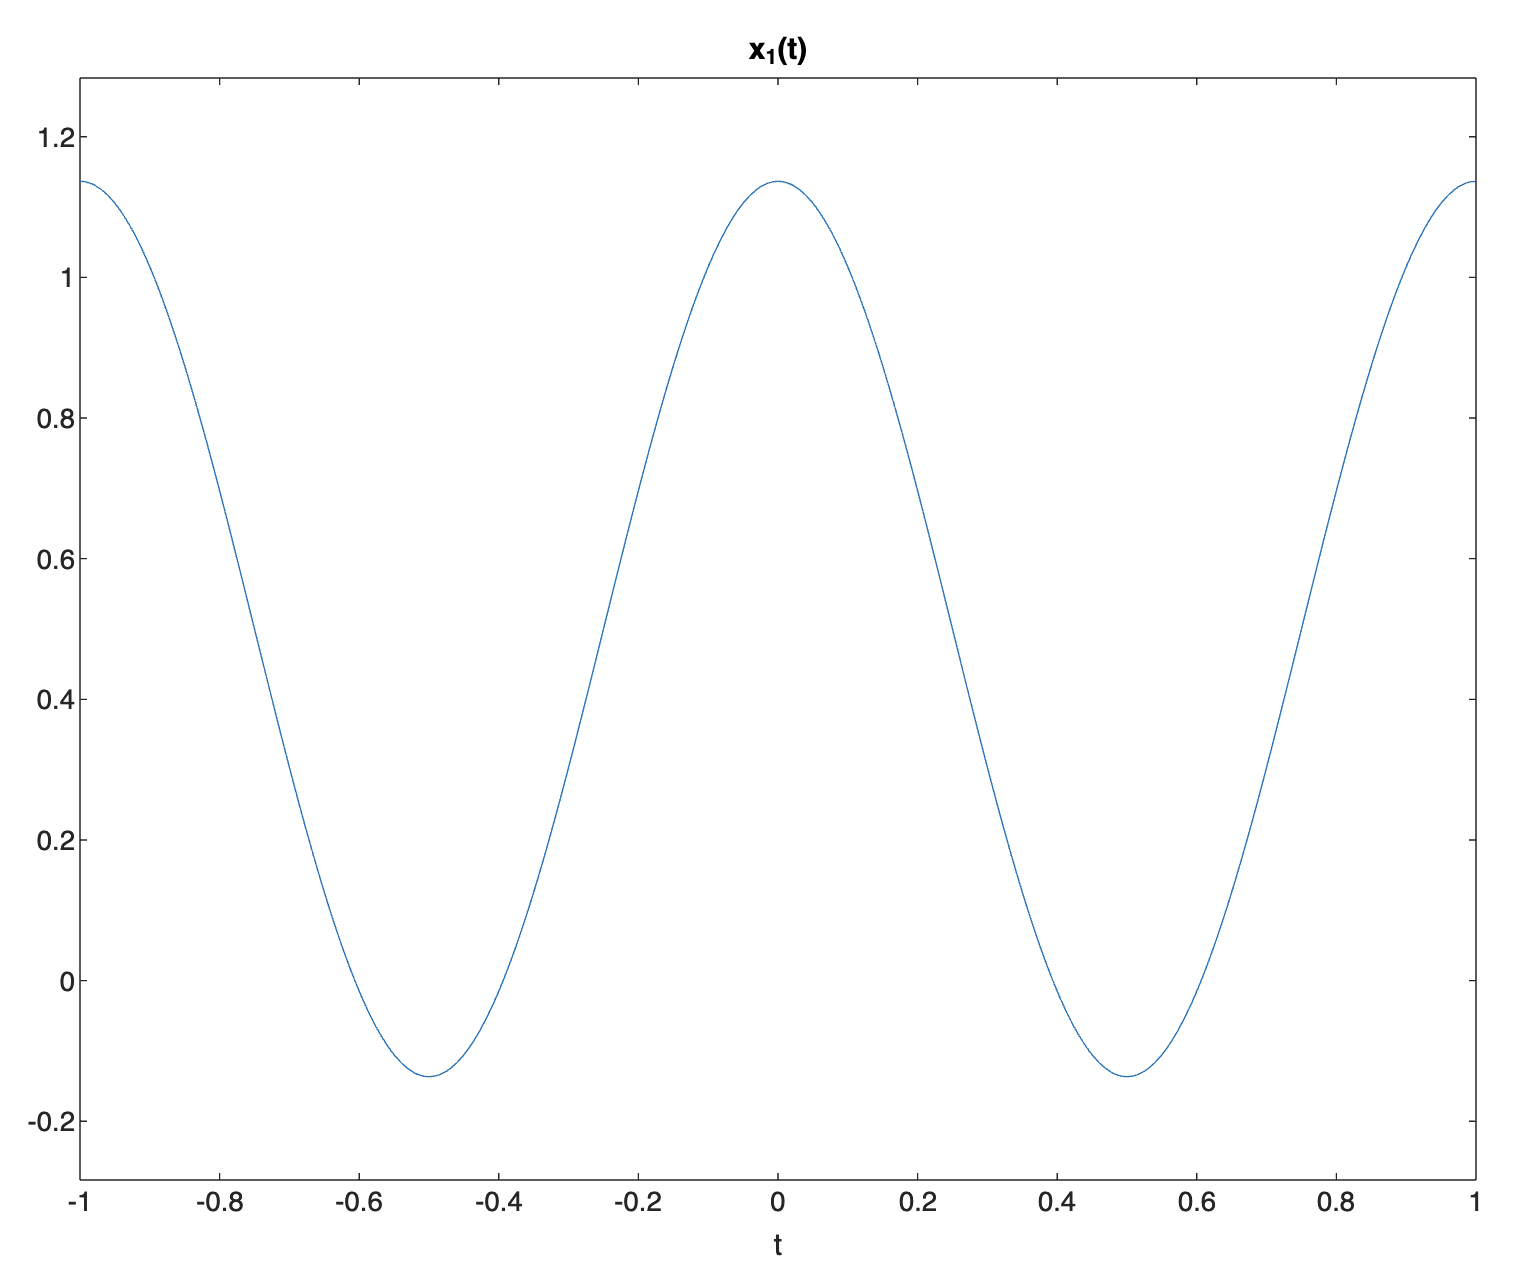
\includegraphics[width=0.8\textwidth]{x1.png}
\end{center}
\begin{center}
    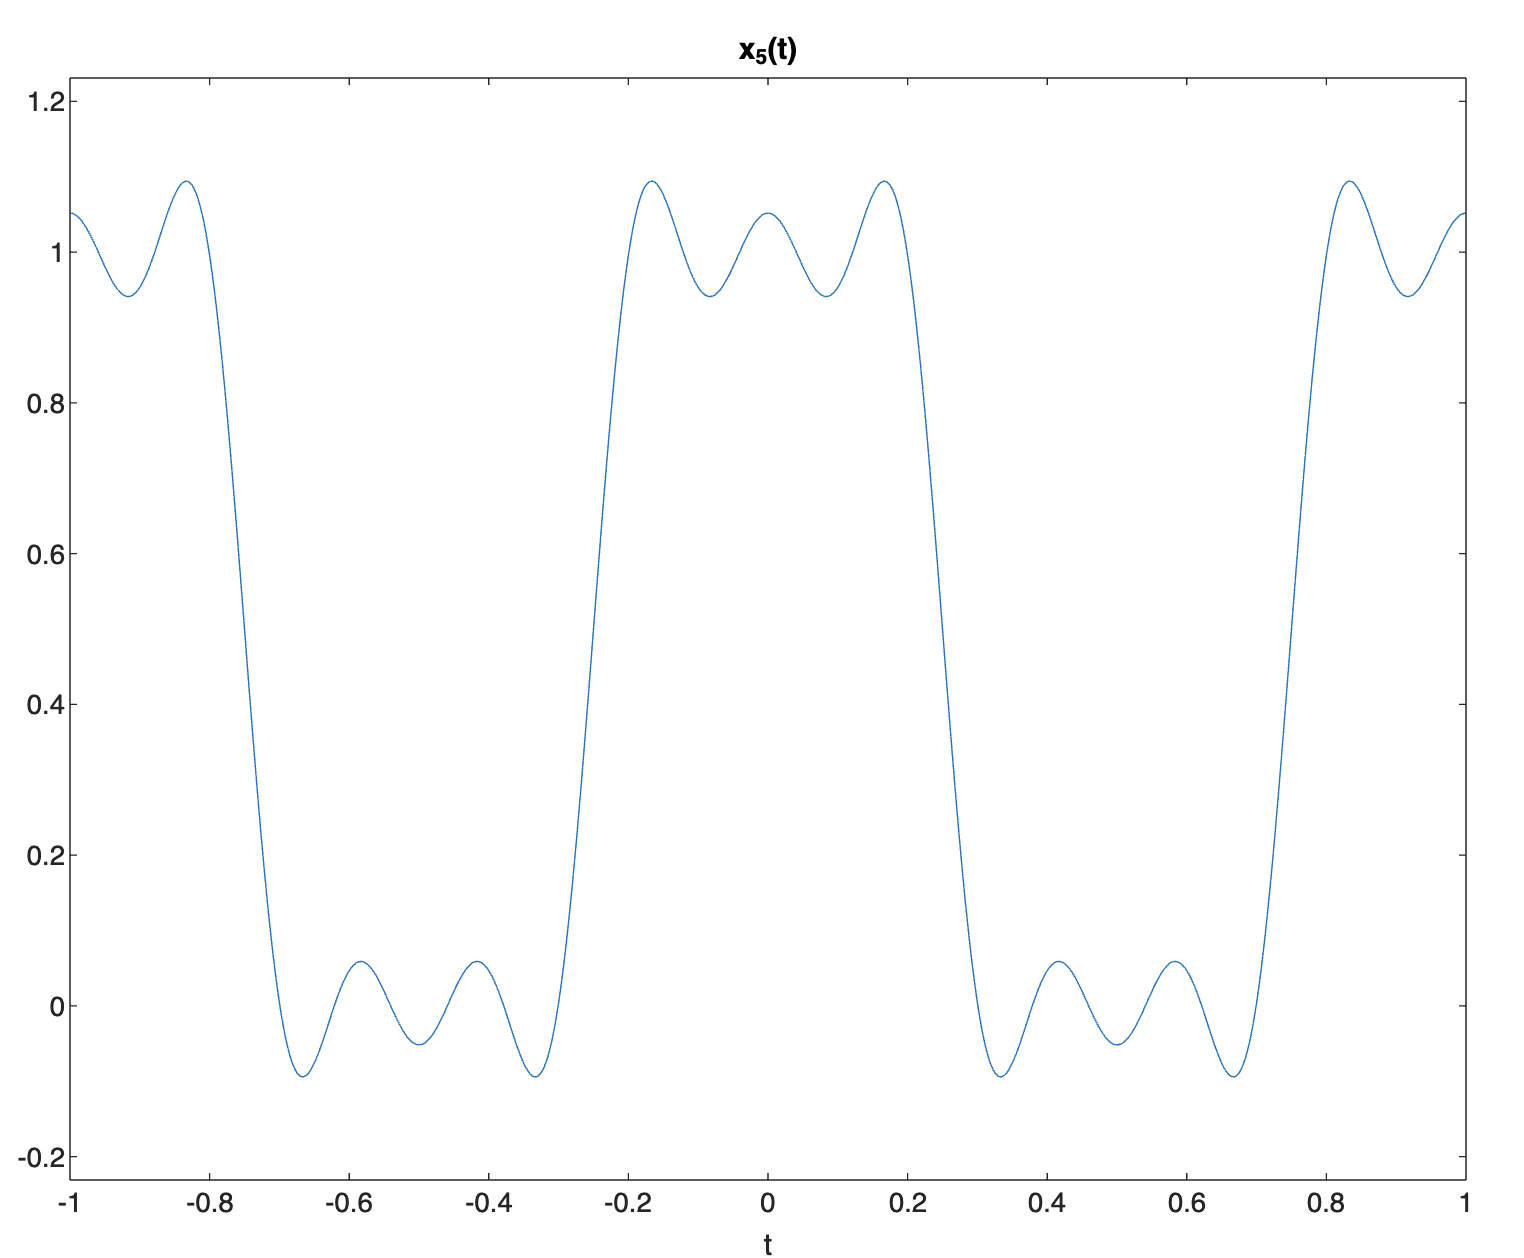
\includegraphics[width=0.8\textwidth]{x5.png}
\end{center}
\begin{center}
    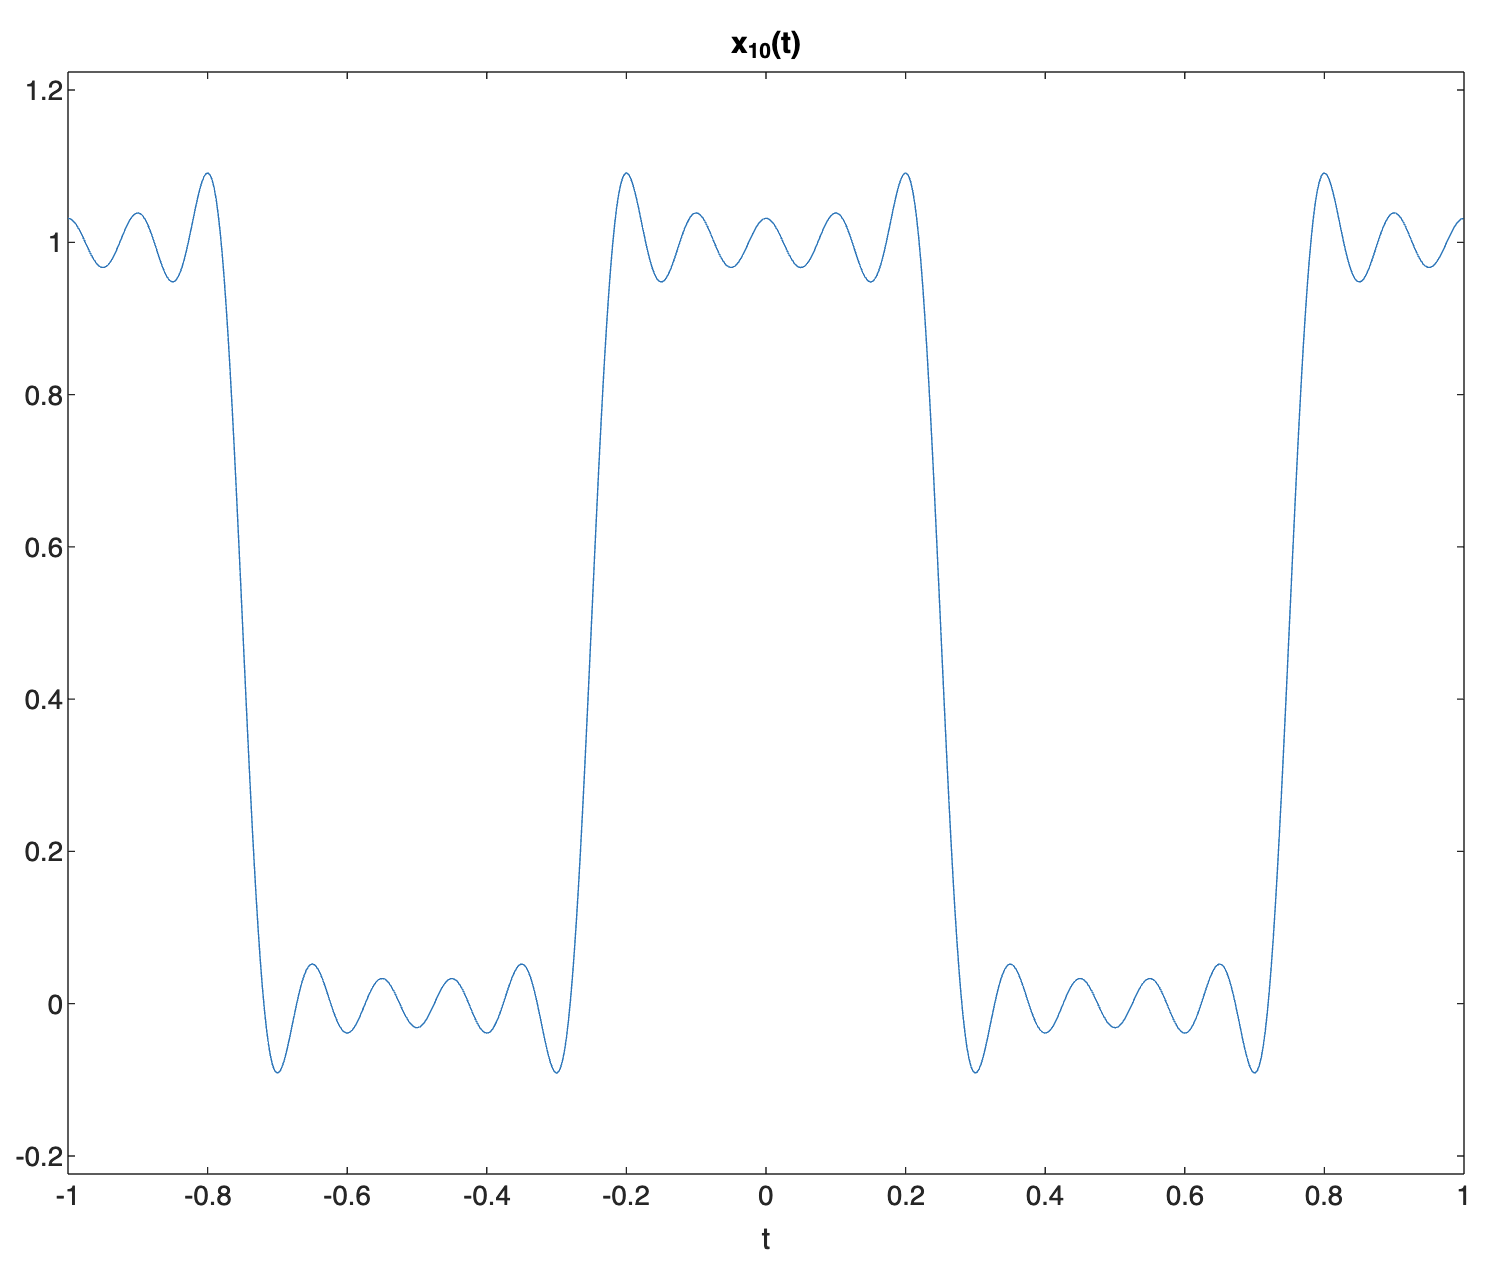
\includegraphics[width=0.8\textwidth]{x10.png}
\end{center}
\begin{center}
    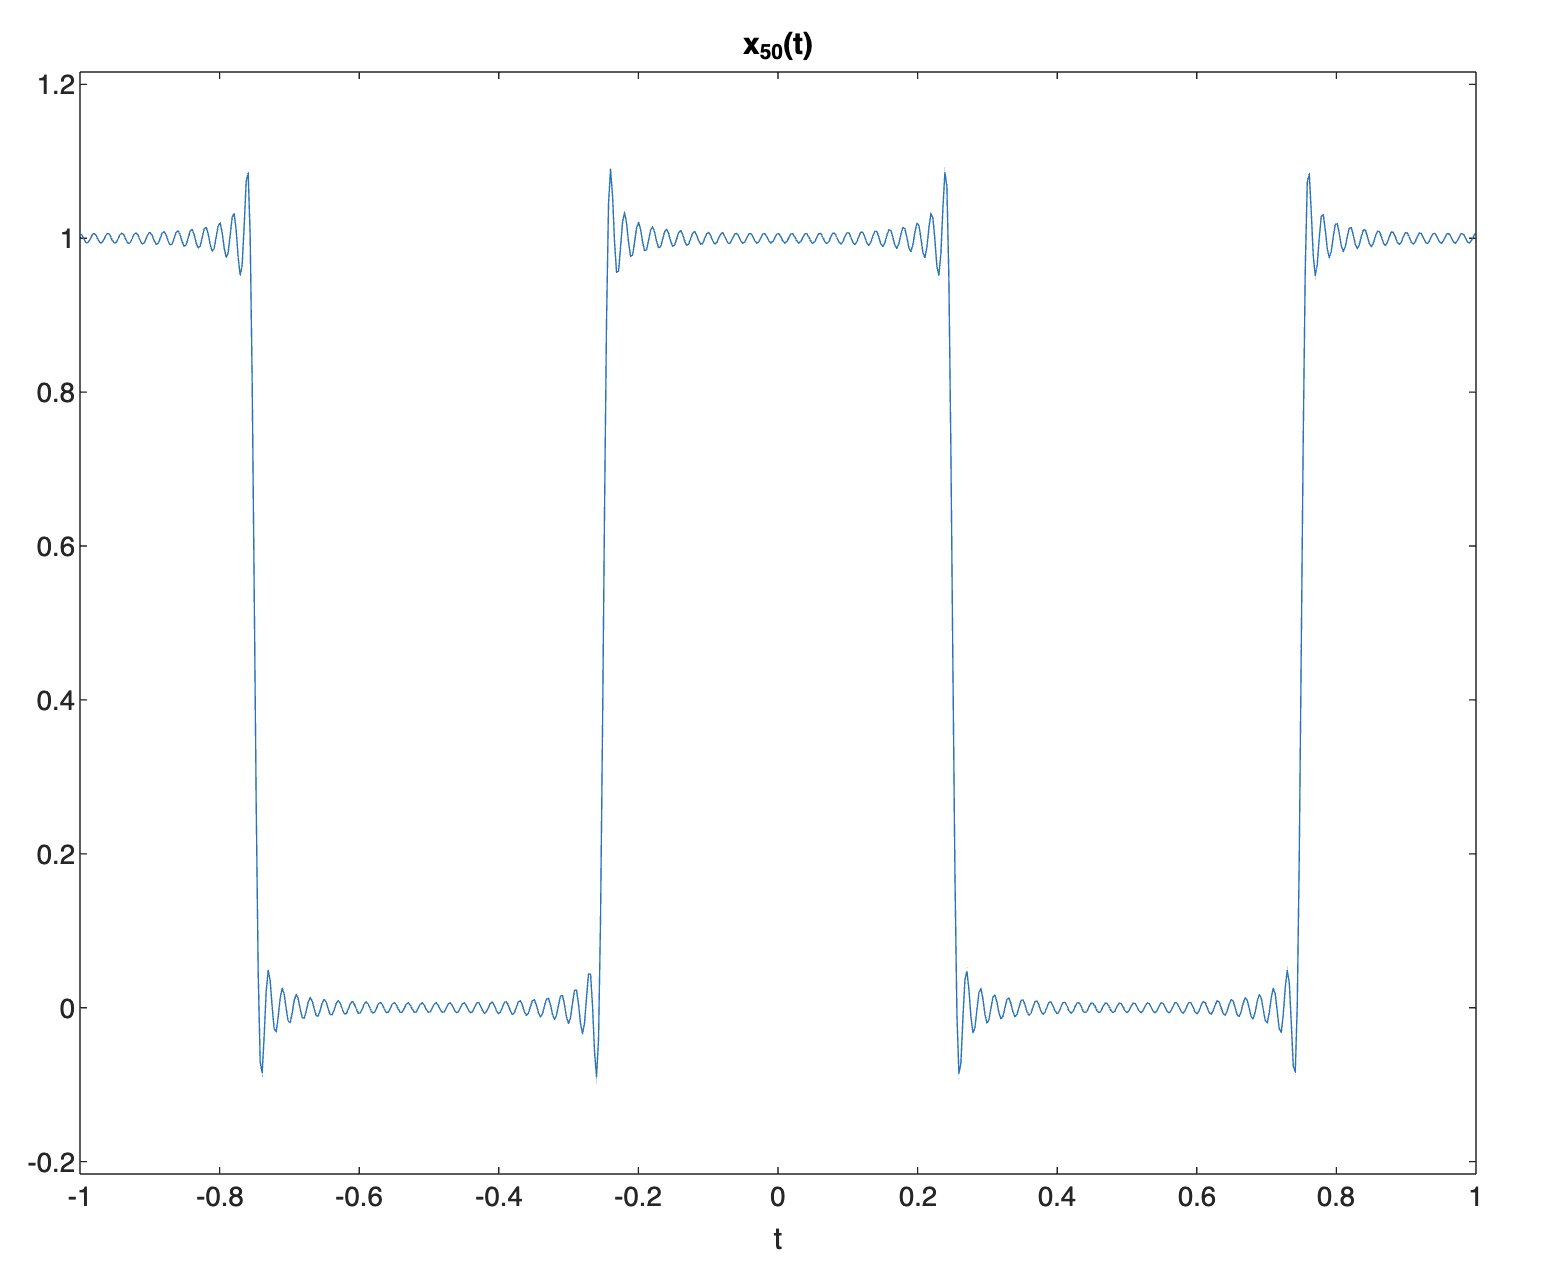
\includegraphics[width=0.8\textwidth]{x50.png}
\end{center}
\begin{center}
    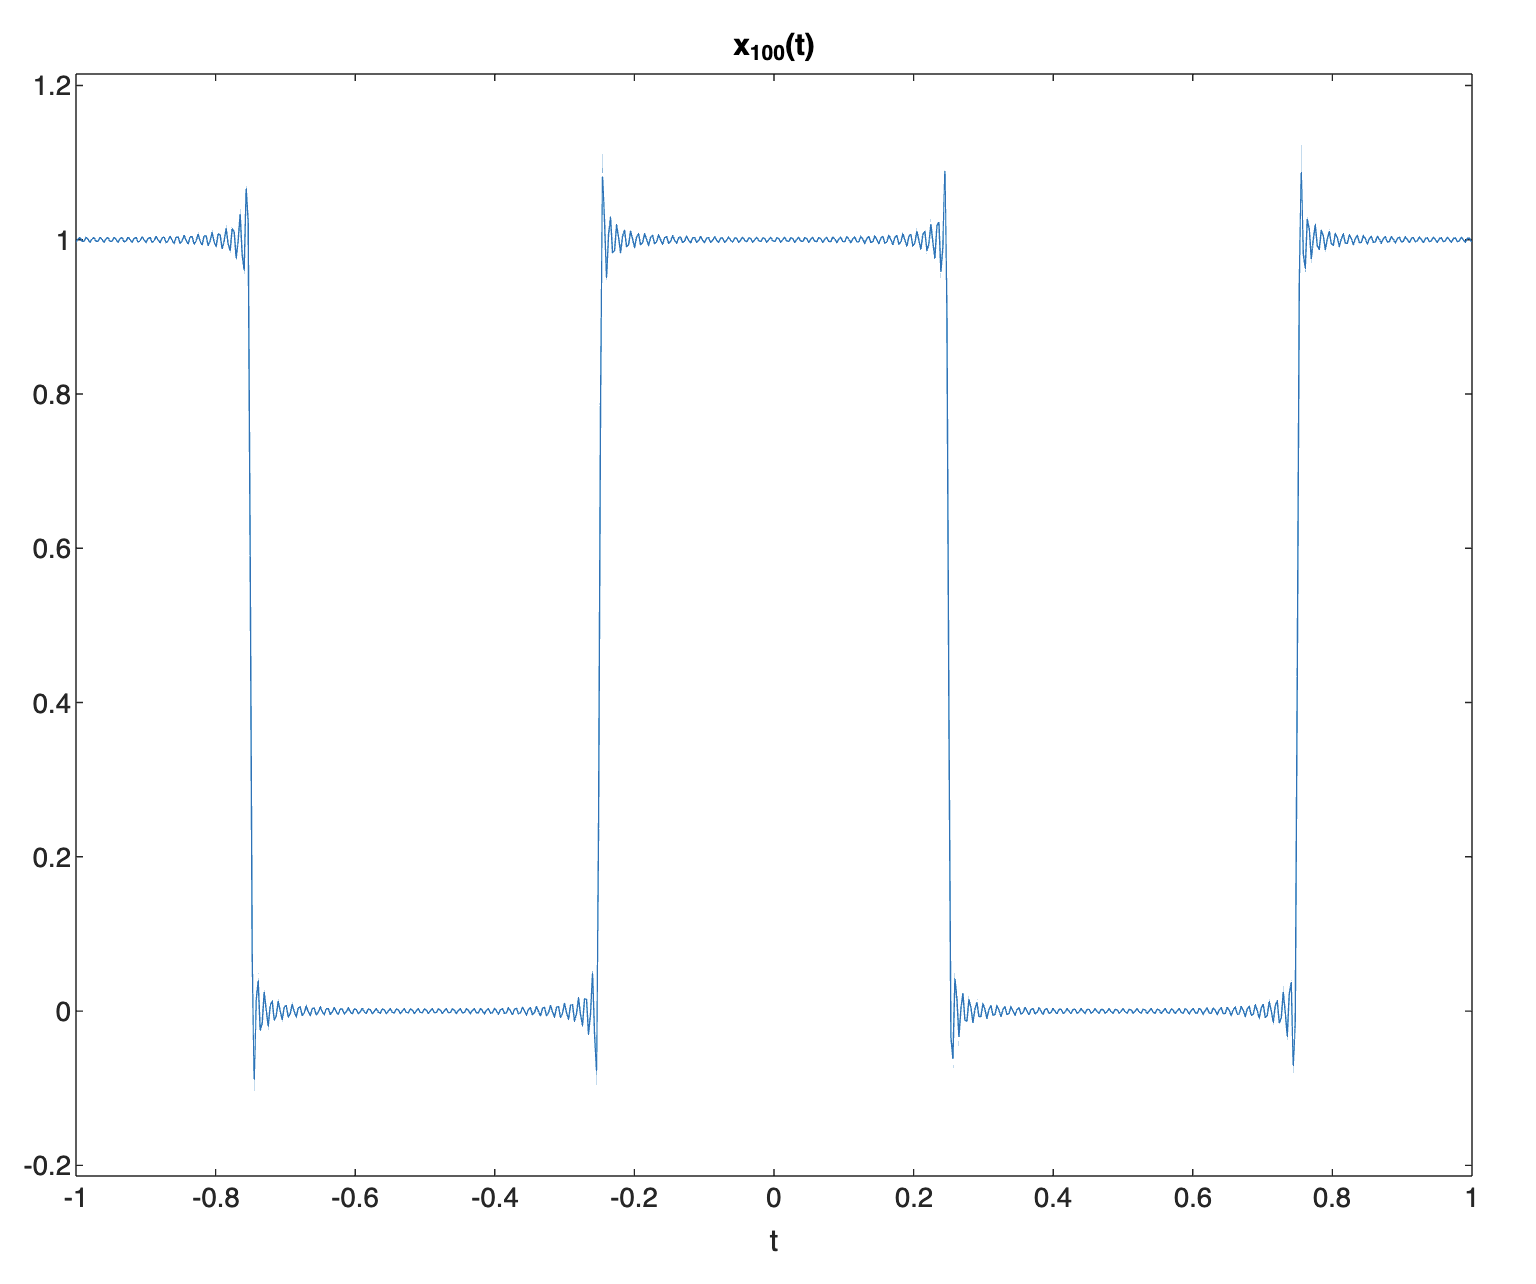
\includegraphics[width=0.8\textwidth]{x100.png}
\end{center}

(b)\\
The function does not converge uniformly everywhere. The function converges at a lower rate at the points of discontinuity.\\

(c)\\
At the point of discontinuity of $x(t)$ at $t = \frac{1}{4}$ the function appears to converge at a value of $\frac{1}{2}$. 





\end{document}
